\documentclass[journal,peerreview,onecolumn]{IEEEtran}
% \documentclass[journal]{IEEEtran}
\usepackage{etex}
\usepackage{cite}
\usepackage[pdftex]{graphicx}
\graphicspath{{./Fig/}}
\DeclareGraphicsExtensions{.pdf,.jpg,.png}
\usepackage{amsmath,amssymb,amsthm}
\usepackage{algorithm}
\usepackage{algorithmic}
\usepackage{array}
\usepackage[caption=false,font=footnotesize]{subfig}
\usepackage{fixltx2e}
\usepackage{url}
\usepackage{listings}
\usepackage{multirow}
\usepackage{tikz}
\usepackage{pgfplots}
\usepackage{tabularx}
\usepackage{empheq}
\usepackage{hyperref}
\usepackage{booktabs}

\newcommand\MyBox[2]{
  \fbox{\lower0.75cm
    \vbox to 1.2cm{\vfil
      \hbox to 1.2cm{\hfil\parbox{1.4cm}{#1\\#2}\hfil}
      \vfil}%
  }%
}

% for peerreview
\usepackage{setspace}
\onehalfspacing

\newtheorem{prop}{Proposition}

% correct bad hyphenation here
% \hyphenation{op-tical net-works semi-conduc-tor}

\begin{document}
%
% paper title
% Titles are generally capitalized except for words such as a, an, and, as,
% at, but, by, for, in, nor, of, on, or, the, to and up, which are usually
% not capitalized unless they are the first or last word of the title.
% Linebreaks \\ can be used within to get better formatting as desired.
% Do not put math or special symbols in the title.
\title{Operational Feature Selection in Gaussian Mixture Models}
%
%
% author names and IEEE memberships
% note positions of commas and nonbreaking spaces ( ~ ) LaTeX will not break
% a structure at a ~ so this keeps an author's name from being broken across
% two lines.
% use \thanks{} to gain access to the first footnote area
% a separate \thanks must be used for each paragraph as LaTeX2e's \thanks
% was not built to handle multiple paragraphs
%

\author{Adrien~Lagrange,~Mathieu~Fauvel~and~Manuel~Grizonnet% <-this % stops a space
\thanks{A. Lagrange and M. Fauvel are with the Université de Toulouse,
INP-ENSAT, UMR 1201 DYNAFOR, France and with the INRA, UMR 1201
DYNAFOR, France.}
\thanks{M. Grizonnet is with Centre Nat. d'Etudes Spatiales, French Space Agency, Toulouse, France.}}

% The paper headers
\markboth{Transactions on Computational Imaging,~Special Issue on Computational Imaging for Earth Sciences, September~2016}{}

% make the title area
\maketitle

\tableofcontents
\clearpage
% As a general rule, do not put math, special symbols or citations
% in the abstract or keywords.
\begin{abstract}
This article presents a forward feature selection algorithm based on Gaussian mixture model (GMM) classifiers. The algorithm selects iteratively features that maximize a criterion function which can be either a classification rate or a measure of divergence. Several variations of this algorithm are explored by changing the criterion function and also by testing a floating forward variation allowing backward step to discard already selected features.

An important effort is made in exploiting GMM properties to implement a fast algorithm. In particular, update rules of the GMM model are used to compute the criterion function with various sets of features. The result is a C++ remote module for the remote sensing processing toolbox Orfeo (OTB) developed by CNES.

Finally, the method is tested and also compared to other classifiers using two different datasets, one of hyperspectral images with a lot of spectral variables and one with heterogeneous spatial features. The results validate the fact that the method performs well in terms of processing time and classification accuracy in comparison to the standard classifiers available in OTB.\\
\end{abstract}

% Note that keywords are not normally used for peerreview papers.
% \begin{IEEEkeywords}
% remote sensing, hyperspectral imaging, feature selection, gaussian mixture model, fast computing.
% \end{IEEEkeywords}

% For peer review papers, you can put extra information on the cover
% page as needed:
% \ifCLASSOPTIONpeerreview
% \begin{center} \bfseries EDICS Category: 3-BBND \end{center}
% \fi
%
% For peerreview papers, this IEEEtran command inserts a page break and
% creates the second title. It will be ignored for other modes.
\IEEEpeerreviewmaketitle

\section{Introduction}
\label{sec:intro}

\IEEEPARstart{W}{ith} the increasing number of remote sensing missions, the quantity of data available for a given landscape becomes larger and larger. Several missions are about to produce huge amount of data or have already produced it. After 2018, the EnMAP (Environmental Mapping and Analysis Program) satellites missioned by the German space agency will produce images with 244 spectral bands with a resolution of 30x30m and revisit every 4 days\cite{Müller09enmap}. The Hyperspectral Infrared Imager (HyspIRI) of NASA will also take images with 212 spectral bands every 5 days. Additionally to hyperspectral data, hypertemporal data are also developping. The European satellites Sentinel-2 were launched successfully recently and the hypertemporal data produced by this mission will be fully available at the end of 2016\cite{drusch2012sentinel}.

However, processing this data is more and more challenging because of statistical and computational issues. This statistical issues are often referred as the \emph{curse of dimensionality}. The Hughes phenomenon \cite{hughes1968mean} states that with a given number of samples, prediction accuracy will decays when the complexity is higher than some optimum value. The problem is the fast increase of the number of parameters to estimate in order to build a model when dimension expands \cite{bouveyron2014model}. Thus, a important number of labeled samples is needed to perform learning. For example, in the case of Gaussian Mixture Models, the number of parameters progresses quadratically with the dimension, e.g. with 200 describing variables, the model estimation requires at least around 20,000 samples by class.

The computational issues are multiple. The computing infrastructure needed to process data is more and more expensive because the processing might requires a GPU and a large amount of RAM to load images which can weight a dozen of gigabytes \cite{christophe2011remote}\cite{plaza2011high}. The processing time is also limiting and requires to use parallelize computing (GPU, multi-threading).

A possible method to solve these issues is to perform a reduction of dimension. It is possible to extract a set of relevant features to get a parsimonious representation of the data \cite{jimenez1998supervised}.

For instance, in land-cover classification, given a set of spatial, temporal and spectral features, it is possible to extract those which are the most discriminant for the purpose of classification \cite{fassnacht2014comparison}. In hyperspectral data analysis from the hundreds of available spectral channels, it is possible to reduce the number of channels to make the processing more efficient in terms of statistical complexity because of the reduction of the number of parameters to estimate and thus also in term of computational time. Moreover, dimensional reduction might improves the capacity of generalization of the classifier and avoid overfitting.

There are two ways to reduce dimension \cite{Guyon:2006:FEF:1208773}: features extraction and feature selection. Feature extraction means creating new features by combining the existing ones, for example linear combination as in Principal Component Analysis \cite{jimenez1998supervised}. To the contrary, features selection selects a subset of existing features. It has the advantage to be much more interpretable for the end-user. The selected subset of features corresponds to the most important features for the given task.

There is a large diversity of methods for feature selection. However, they usually do not scale well with the number of pixels to be processed \cite{fauvel2015fast}. Nevertheless, methods based on Gaussian Mixture Models (GMM) have several interesting properties that make them suitable for feature selection in the context of large amount of data. By taking advantage of their intrinsic properties, it is possible to increase the computational efficiency with respect to standard implementation.

Several strategy have been explored to perform feature selection and, among them, wrapper methods receive a certain interest of the community. Wrapper methods can be seen as a search method to determine the best subset of variables for a given learning model. As exhaustive searches are out of question in a practical amount of time, numerous search strategies have been designed. Some optimal are under particular hypothesis \cite{narendra1977branch} and other suboptimal but easier to set up \cite{whitney1971direct}\cite{somol1999adaptive}. Such methods have the advantage to tune the selection to make the most of a particular classifier but require the training of multiple models to test various set of variables which can make them slow if the training is not optimized.

This work proposes to develop a forward feature selection method using GMM in continuation of \cite{fauvel2015fast} and an upgraded floating forward method. The basic method selects iteratively the meaningful features. At each step, the pool of selected features is used to train a GMM which allows to compute a criterion function then used to rank features at the next iteration. The upgraded method introduces possible backward steps after each addition of a feature. An efficient implementation of the method is presented in order to handle large amount of data. Moreover, the developed algorithm is made available as a remote module of the C++ Orfeo Toolbox \cite{christophe2008orfeo}. Finally, tests are conducted to compare different variations of the method and to compare also to other classifiers (GMM, Random Forest, k-nearest-neighbor) available in the Orfeo Toolbox.

The remaining of this article is organized as follows. Section~\ref{sec:gmm-hd} presents Gaussian Mixture Model classifiers and the features selection methods used to make them suitable for high-dimension space. The work done to develop a smart implementation of the proposed selection method is presented in Section~\ref{sec:implementation}. And finally, the tests conducted to explore variations of the algorithm and to compare it to other standard classifiers are detailed in Section~\ref{sec:test}.

\section{Gaussian Mixture Models in high dimensional space}
\label{sec:gmm-hd}

The    following    notations    are   used    in    the    remaining.
$\mathcal{S}  = \{\mathbf{x}_i,y_i\}_{i=1}^{n}$  denotes the  training
set where $\mathbf{x}_i \in \mathbb{R}^d$ is the vector of features of
the $i^{th}$ sample, $y_i = 1,...,C$ the associated label, C the total
number of classes,  $n$ the number of samples and  $n_c$ the number of
samples of class $c$.

    \subsection{Gaussian Mixture Models}

    For mixture models, it is assumed  that a given sample $\mathbf{x}$ is
    the realization  of a  random vector which  distribution is  a mixture
    (convex     combination)     of      several     class     conditioned
    distribution~\cite{Fraley00model-basedclustering}:
    \begin{equation}
        p(\mathbf{x}) = \sum_{c=1}^{C} \pi_c f_c(\mathbf{x}|\theta)
    \end{equation}
    where $\pi_c$ is  the prior, \emph{i.e.}, the  proportion of class
    $c$  and  $f_c$  a  parametric density  function  parametrized  by
    $\theta$.

    Among the possible parametric model,  the Gaussian one is the most
    used~\cite{bouveyron2014model}.   It assumes  that each  $f_c$ is,
    conditionally  to  $c$,  a  Gaussian  distribution  of  parameters
    $\boldsymbol{\mu}_c$    and    $\boldsymbol{\Sigma}_c$:
    \begin{equation*}
        f_c(\mathbf{x}|\boldsymbol{\mu}_c, \boldsymbol{\Sigma}_c) = \frac{1}{(2\pi)^{\frac{d}{2}} |\boldsymbol{\Sigma}_c|^{\frac{1}{2}}} \exp \left( -\frac{1}{2} (\mathbf{x} - \boldsymbol{\mu}_c)^t \boldsymbol{\Sigma}_c^{-1} (\mathbf{x} - \boldsymbol{\mu}_c) \right).
    \end{equation*}

    It  is  referred  to  as  Gaussian  mixture  model  (GMM).   In  a
    supervised    learning    framework,    the    class    parameters
    $\boldsymbol{\mu}_c$,   $\boldsymbol{\Sigma}_c$   and  the   prior
    $\pi_c$ are  usually estimated  through the  conventional unbiased
    empirical estimators:
    \begin{align}
        \hat{\pi}_c &= \frac{n_c}{n},\\
        \hat{\boldsymbol{\mu}}_c &= \frac{1}{n_c} \sum_{\{i|y_i = c\}} \mathbf{x}_i ,\\
        \hat{\boldsymbol{\Sigma}}_c &= \frac{1}{(n_c - 1)} \sum_{\{i|y_i = c\}} (\mathbf{x}_i - \boldsymbol{\mu}_c) (\boldsymbol{}x_i - \boldsymbol{\mu}_c)^t.
    \end{align}

    To predict the  class of a new unseen sample,  the maximum \emph{a
      posteriori}  rule  is  used:
    \begin{equation*}
        \mathbf{x} \text{ belongs to } c \Leftrightarrow c = \text{arg} \max_{c \in C} p(c) p(\mathbf{x}|c).
    \end{equation*}
    Under the GMM,  and identifying $p(c)$ as $\pi_c$  and $p(x|c)$ as
    $f_c(x|\theta)$ and by taking the log, a decision rule is obtained
    \begin{eqnarray}\label{eq:decision}
      Q_c(\mathbf{x}) &=& 2 \log \left( p(c) p(\mathbf{x}|c) \right) \nonumber \\
                      &=& - (\mathbf{x} - \boldsymbol{\mu}_c)^t \boldsymbol{\Sigma}_c^{-1} (\mathbf{x} - \boldsymbol{\mu}_c) \nonumber \\
                      & &-\log (|\boldsymbol{\Sigma}_c|) + 2 \log (\pi_c) - d \log (2\pi).
    \end{eqnarray}

    \subsection{Curse of dimensionality in GMM}
    \label{sec:curse:gmm}

    The computation of~\ref{eq:decision} requires the inversion of the
    covariance matrix and and the  computation of the logarithm of the
    determinant.  The estimations of these terms suffer from the curse
    of  dimensionality\cite{bouveyron2014model}, because  in practice,
    the  number of  parameters  $\eta_c$ to  estimate  for each  class
    increases quadratically with respect to the number of features, as
    illustrated in Figure~\ref{fig:nb-param}.  Hence, if the number of
    observation  $n_c$ is  small  compared to  the  number of  samples
    $n_c$, the  estimated covariance  matrix is badly  conditioned and
    thus the computation  of its inverse and its  determinant would be
    unstable.   The worst  situation  is $n_c<\eta_c$  which leads  to
    singular covariance matrix.  Unfortunately, this situation happens
    regularly in remote sensing.   For instance in hyperspectral image
    classification,  very few  labeled samples  are usually  available
    because of the difficulty and the cost to collect ground-truth.

    \begin{figure}[!t]
        \centering
        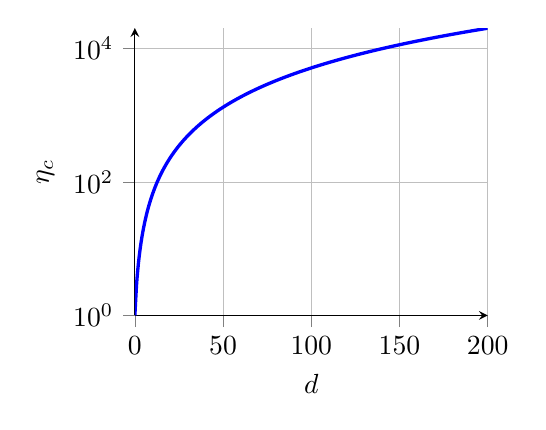
\begin{tikzpicture}
          \begin{semilogyaxis}[xmin=0,xmax=200,ymin=0,width=0.5*\columnwidth,grid,axis x line=left ,axis y line=left, tick align=outside,xlabel = $d$,ylabel = $\eta_c$]
            \addplot+[very thick,mark=none,smooth,domain=0:200,samples=200] (\x,{\x*(\x+3)/2+1});
            \end{semilogyaxis}
        \end{tikzpicture}
        \caption{Number of parameters $\eta_c$ by class in function of dimension $d$: $\eta_c=d(d+3)/2+1$.\label{fig:nb-param}}
    \end{figure}

    %% TODO: il faut reprendre cette partie en détaillant plus
    %% Il y a deux approches: une qui regularise le probleme inverse,
    %% ridge est une solution, mais il y en a d'autres. Voir le
    %% paragraphe qui est consacré à cela dans la thèse d'Anthony ->
    %% elle arrive pas mail. Ensuite, il y a la réduction de dimension
    %% données des refs (voir intro du papier JSTARS) et dans la
    %% réduction  de dimension, il  y a  la sélection de  features. La
    %% conclusion doit s'enchainer avec la partie suivante.
    There are two major  solutions to this problem. First option is to stabilize the inversion of the covariance matrices work. Some methods investigate the use of constraints on the direct problem \cite{reynolds1995robust} \cite{hathaway1985constrained} and some work on the inverse problem by using regularization method \cite{hoerl1970ridge} \cite{jensen2008regression}. Second option is to reduce dimension. Features extraction/selection methods have been developed in order to reduce the dimension. In this  study, the latter option is explored and a feature selection method named sequential forward features selection is presented after a brief overview of the selection algorithms in the next Section. %A finir

\section{Sequential forward features selection}
\label{sec:selection}

%%% Debut Déplacer vers l'intro
The objective of feature selection is to retrieve the most compact representation of the data with minimum loss of information \cite{Guyon:2006:FEF:1208773}. By deleting the redundant information, feature selection allows to reduce dimension and thus avoid statistical issue, increase algorithm speed and limit storage requirements. Moreover, it adds several beneficial side effects. It improves data understanding by identify where is the most relevant information and it is then possible to save resources when organizing a new data acquisition.% TODO: add ref. et example

%% Cette partie, dans l'intro il faut la rallonger: mieux décrire ces trois méthodes, dire les avantages et les inconvénients de chaque approche et positionner notre approche par rapport à tout cela (je dis cela sans avoir relu l'intro). Tu peux t'inspirer de la thèse de Arnaud Lebris et des pages 58-66)
Features selection algorithms can be divided into three types. The first type, called \emph{filter methods}, is based uniquely on data analysis. Features are ranked according to a statistical analysis of the data. For example, the Principal Component Analysis (PCA) described in \cite{jimenez1998supervised} is a typical filter method and there is numerous other methods \cite{bruzzone1995extension,biesiada2007feature,demir2008phase}.

The second sort are known as \emph{wrapper methods} which can be seen as search method to determine the best subset of variables for a given learning model. As exhaustive searches are to expansive in terms of processing time, several search strategies have been designed. Some are optimal under particular hypothesis \cite{narendra1977branch} and other sub-optimal but easier to set up \cite{whitney1971direct,somol1999adaptive}. The advantage of such methods compare to filter methods is that they are dedicated to a particular model but on the other hand, as they require the training of multiple models to test various set of variables, they tend to be more time consuming.

The third type corresponds to the \emph{embedded method} which do not separate the features selection process from the learning algorithm and allow interaction between the two processes. The basic example of such method is the decision tree algorithm in which a feature is selected for the creation of each node. Embedded methods also exist for other models, e.g. SVM \cite{guyon2002gene,weston2003use}.
%%% Fin déplacer

The feature selection method proposed in this work is a wrapper method associated to GMM models. Two elements are needed to set up a wrapper method:
\begin{enumerate}
\item A function that  ranks the features according to some good classification criteria,
\item A search strategy to optimize the function.
\end{enumerate}

Section~\ref{sec:criterion} describes the different criterion used in this work and two search strategies are discussed in~\ref{sec:selection:method}.


    \subsection{Criterion function}
    \label{sec:criterion}
    The criterion evaluates how a given model built with a subset of features performs for the classification task. It can be an estimation of the correct classification or a measure of separability/similarity between class distribution. The former are in general more demanding in terms of processing time than the later.
    
    % Criterion functions aim to evaluate either a rate of correct classification or the separability/similarity of class distributions. These functions are used to estimate which sets of variables are the best to represent data, to assure the separability of the classes and to perform classification. The choice of a criterion function is the choice of a way to compare sets of variables.

        \subsubsection{Measures of correct classification}
        \label{sec:criterion-rate}

        A measure of correct classification is based on an error matrix $M$, or \emph{confusion matrix}~\cite[Chapter 4]{congalton2008assessing}. An element $M_{ij}$ of the matrix represents the number of samples of class $i$ classified as class $j$. The confusion matrix allows the computation of several global and per-class indices related to the classification accuracy~\cite{congalton2008assessing}. Three global criteria were used 
        \begin{itemize}
        \item  \emph{The overall  accuracy} (OA)  is the  rate of  the
          number of samples with the  correct predicted label over the
          total  number of  samples~\cite{congalton2008assessing}. This
          metric is  easy to interpret  but is  biased in the  case of
          unbalanced classes.

        \item \emph{The Cohen's kappa} (K) is a statistic which measures the probability of agreement between predictions and ground-truth~\cite{congalton2008assessing}.

        \item \emph{The mean F1 score}  (F1mean) is the average of the
          F1 score  for each class  and the  F1 score is  the harmonic
          mean of  the precision  (number of  True Positive  over True
          Positive plus False Positive) and the recall (number of True
          Positive over True Positive plus False Negative)~\cite{powers2011evaluation}.
      \end{itemize}
      
      The classification rate is  estimated by a $k$- cross-validation
      ($k$-CV)~\cite{opac-b1127878}.  To compute  the $k$-CV, a subset
      is removed  from $\mathcal{S}$ and  the GMM is learned  with the
      remaining training samples.   A test error is  computed with the
      removed  training  samples  used  as  validation  samples.   The
      process is  iterated $k$ times and  the estimated classification
      rate is computed as the mean  test error over the $k$ subsets of
      $\mathcal{S}$.

        \hspace{0pt} \\

        \subsubsection{Similarity between distributions}
        These measures are called divergence function and are defined so that, if $S$ is a space of all probability distribution with same support, it satisfies
        \begin{align*}
            &\forall (p,q) \in S, \text{Div}(p,q) \geq 0, \\
            &\text{Div}(p,q) = 0 \Leftrightarrow p = q.
        \end{align*}
        More specifically, focus is made on two particular divergences: the Kullback–Leibler divergence and the Jeffries–Matusita distance. The advantage of these divergences is that they have an explicit expression in the case of Gaussian models. The simplification allows to get rid of any integration calculus which is a major problem when dealing with high-dimensional data.


        \emph{The Kullback-Leibler divergence} (KL divergence) measures the amount of information lost when the first distribution is approximated by the second one\cite{kullback1987letter}. The formal definition is
        \begin{equation}
            \text{Div}_{KL}(c_i,c_j) = \int_\mathbf{x} p(\mathbf{x}|c_i) \ln \left(\frac{p(\mathbf{x}|c_i)}{p(\mathbf{x}|c_j)}\right) d\mathbf{x}.
        \end{equation}
        And in the case of Gaussian model, it can be rewritten as follows
        \begin{align}
            &\text{Div}_{KL}(c_i,c_j) = \frac{1}{2} \biggl( \text{Tr} (\boldsymbol{\Sigma}_{c_i}^{-1} \boldsymbol{\Sigma}_{c_j}) \nonumber \\
            & + (\boldsymbol{\mu}_{c_i} - \boldsymbol{\mu}_{c_j})^t \boldsymbol{\Sigma}_{c_i}^{-1} (\boldsymbol{\mu}_{c_i} - \boldsymbol{\mu}_{c_j}) - d + \log \left( \frac{|\boldsymbol{\Sigma}_{c_i}|}{|\boldsymbol{\Sigma}_{c_j}|} \right) \biggr),
        \end{align}
        where Tr is the trace operator and $d$ the dimension of the distribution.

        It can be noticed that the KL divergence is not symmetric, i.e. $\text{Div}_{KL}(c_i,c_j) \ne \text{Div}_{KL}(c_j,c_i)$, and so the symmetrized version is used to compute the criterion function. In the case of Gaussian model, the symmetrization induces the following simplification of the formula
        \begin{align}
            \text{SKL}_{ij} &=\text{Div}_{KL}(c_i,c_j) + \text{Div}_{KL}(c_j,c_i) \nonumber \\
            &= \frac{1}{2} \biggl( \text{Tr} (\boldsymbol{\Sigma}_{c_i}^{-1} \boldsymbol{\Sigma}_{c_j} + \boldsymbol{\Sigma}_{c_j}^{-1} \boldsymbol{\Sigma}_{c_i}) \nonumber \\
            &~~+ (\boldsymbol{\mu}_{c_i} - \boldsymbol{\mu}_{c_j})^t (\boldsymbol{\Sigma}_{c_i}^{-1} + \boldsymbol{\Sigma}_{c_j}^{-1}) (\boldsymbol{\mu}_{c_i} - \boldsymbol{\mu}_{c_j}) - 2d \biggr).
        \end{align}

        Moreover, the divergence is computed between two classes and to obtain a unique value the weighted mean of divergence measures is taken as proposed in \cite{bruzzone1995extension}:
        \begin{equation}
            \text{C}_{SKL} = \sum_{i=1}^{C} \sum_{j=i + 1}^{C} \pi_{c_i} \pi_{c_j} \text{SKL}_{ij}.
        \end{equation}

        \emph{The Bhattacharyya distance} is defined as follows
        \begin{equation}
            \text{B}_{ij} = - \ln \left( \int_\mathbf{x} \sqrt{p(\mathbf{x}|c_i) p(\mathbf{x}|c_j)} d\mathbf{x} \right).
        \end{equation}
        And in the case of Gaussian model:
        \begin{align}
            \text{B}_{ij} = &\frac{1}{8} (\boldsymbol{\mu}_i - \boldsymbol{\mu}_j)^t \left( \frac{\boldsymbol{\Sigma}_i + \boldsymbol{\Sigma}_j}{2} \right)^{-1} (\boldsymbol{\mu}_i - \boldsymbol{\mu}_j) \nonumber \\
            &+ \frac{1}{2} \ln \left( \frac{|\boldsymbol{\Sigma}_i + \boldsymbol{\Sigma}_j|}{\sqrt{|\boldsymbol{\Sigma}_i| |\boldsymbol{\Sigma}_j|}} \right).
        \end{align}

        \emph{The Jeffries–Matusita distance} is a measure based on the Bhattacharyya distance. It saturates if the separability between the two distribution increases \cite{bruzzone2009novel}. The JM distance is defined according to
        \begin{equation}
            \text{JM}_{ij} = \sqrt{ \int_\mathbf{x} \left[\sqrt{p(\mathbf{x}|c_i)} - \sqrt{p(\mathbf{x}|c_j)}\right]^2 d\mathbf{x} }.
        \end{equation}
        And the Jeffries–Matusita distance can be rewritten according to the Bhattacharyya distance
        \begin{equation}
            \text{JM}_{ij} = \sqrt{ 2 \{1 - \text{exp}[-B_{ij}]\} }.
        \end{equation}

        As for the KL divergence, a weighted mean of the distance between two classes is computed to aggregate the measures in a single value:
        \begin{equation}
            \text{C}_{JM} = \sum_{i=1}^{C} \sum_{j=i + 1}^{C} \pi_{c_i} \pi_{c_j} \text{JM}_{ij}.
        \end{equation}

        \vspace{10 mm}

        According to \cite{bruzzone2009novel}, it is interesting to notice that the KL divergence increases quadratically with respect to the distance between the mean vectors of the class distributions whereas the measures of correct classification asymptotically tends to one when distributions are perfectly separable. On the contrary, the JM distance tends to saturate as the measures of correct classification. Table~\ref{tab:crit} summarized the presented criterion functions and their characteristics.

        \begin{table}[!t]
            \centering
            \caption{Summary of the different criterion functions.\label{tab:crit}}
            \begin{tabular}[b]{lccc}
              \toprule
              Criterion & Type Divergence & Complexity \\
              \midrule
              Overall accuracy            & Accuracy   & High \\
              Cohen's kappa               & Accuracy   & High\\
              F1 mean                     & Accuracy   & High\\
              \midrule
              Kullback-Leibler divergence & Divergence & Low \\
              Jeffries-Matusita distance  & Divergence & Low \\
              \bottomrule
            \end{tabular}
        \end{table}

        \subsection{Selection method}
        \label{sec:selection:method}

        \subsubsection{Sequential forward features selection}
        \label{sec:forward-presentation}

        The Sequential Forward Selection (SFS) starts with an empty set of selected features. Then, it computes at each step for all the remaining features the value of the criterion function $J$ chosen among the ones presented in Table~\ref{tab:crit} when the feature is added to the pool of selected features. The feature that maximizes the criterion function is definitively added to the pool of selected features and it moves to the next iteration. The algorithm stops when a given number of variables \emph{maxVarNb} has been selected. The Algorithm~\ref{alg:sfs} presents the process in details.

        The advantage of this search algorithm is its reasonable processing time. The trade-off is that the result is a suboptimal solution in the sense that an untested subset of variable could lead to better classification result.

        \begin{algorithm}
        \caption{Sequential forward features selection\label{alg:sfs}}
        {\footnotesize
        \begin{algorithmic}[1]
        \REQUIRE $\Omega,J,\text{maxVarNb}$
        \STATE $\Omega=\emptyset$
        \STATE $F=\text{\{all variables\}}$
        \WHILE{$\text{card}(\Omega) \leq maxVarNb$}
        \FORALL{$f_i \in F$}
        \STATE $R_i = J(\{\Omega + f_i\})$
        \ENDFOR
        \STATE $j=\text{arg} \max_{i} R_i$
        \STATE $\Omega = \{\Omega + f_j\}$
        \STATE $F = F \setminus f_j$
        \ENDWHILE
        \RETURN $\Omega$
        \end{algorithmic}
        }
        \end{algorithm}

        \subsubsection{Sequential floating forward feature selection}
        \label{sec:floating-presentation}

        The Sequential Floating Forward Selection (SFFS)\cite{somol1999adaptive} is actually based on two algorithms: the SFS described above and the Sequential Backward Selection (SBS). The SBS is the backward equivalent of SFS. The difference is that it starts with every features in the pool of selected features and tries at each step to remove the less significant one in term of the given criterion function.

        The SFFS works as the SFS but between each step of the SFS algorithm a backward selection is operated. At the end of the SBS step, the value of the criterion function is compared to the best value ever obtained with a set of features of the same size and if the new value is better the feature put into question is effectively taken away and the next step is again a SBS but if the new value is not better the SBS step is forgotten and it moves to the next SFS step. The algorithm stops when a given number of features \emph{maxVarNb} has been selected. The Algorithm~\ref{alg:sffs} sums up the method.

        This SFFS algorithm eventually tests more solutions than the SFS algorithm. The results are expected to be better but the trade-off is an increased computational time which is dependent on the complexity of the dataset.

        \begin{algorithm}
        \caption{Sequential floating forward features selection\label{alg:sffs}}
        {\footnotesize
        \begin{algorithmic}[1]
        \REQUIRE $J,\text{maxVarNb}$
        \STATE $\Omega=\overbrace{(\emptyset,...,\emptyset)}^{maxVarNb}$
        \STATE $F=\text{\{all variables\}}$
        \STATE $k=0$
        \WHILE{$k \neq \text{maxVarNb}$}
        \FORALL{$f_i \in F$}
        \STATE $R_i = J(\{\Omega_k + f_i\})$
        \ENDFOR
        \STATE $j=\text{arg} \max_{i} R_i$
        \STATE $k=k+1$
        \IF{$R_j \geq J(\Omega_k)$}
        \STATE $\Omega_k = \{\Omega_{k-1} + f_j\}$
        \STATE $\text{flag}=1$
        \WHILE{$k > 2 \text{ and } \text{flag}=1$}
        \FORALL{$f_i \in \Omega_k$}
        \STATE $R_i = J(\{\Omega_k \setminus f_i\})$
        \ENDFOR
        \STATE $j=\text{arg} \max_{i} R_i$
        \IF{$R_j > J(\Omega_{k-1})$}
        \STATE $\Omega_{k-1} = \{\Omega_k \setminus f_j\}$
        \STATE $k=k-1$
        \ELSE
        \STATE $\text{flag}=0$
        \ENDIF
        \ENDWHILE
        \ENDIF
        \ENDWHILE
        \RETURN $\Omega_{\text{maxVarNb}}$
        \end{algorithmic}
        }
        \end{algorithm}


\section{Efficient implementation}
\label{sec:implementation}

    \subsection{Statistical update rules}
    In the presented method, the most costly operation is the evaluation of the criterion function which needs to be done for each possible subset of variables augmented by one of the candidate variable. To compute these values, the most costly operation are the inversion of the covariance matrix and the computation of its determinant. Both of these operations have a $O(n^3)$ computational complexity. Additionaly, the estimation of classification rate with cross-validation is a heavy process which take a consequent amount of time.

    A major contribution of this work is the optimization in term of computational efficiency. More precisely, three steps of the proposed method has been upgraded in order to reduce computational time. First of all, the GMM model is learned only once using samples. When a covariance matrix or a mean vector of a reduced set of variables is required, it is obtained from the global model learned at the beginning by marginalization.

    Secondly, when a cross-validation is performed, submodels, i.e. GMM model trained with $(n_{cv}-1)$ folds, are not learned using the $(n_{cv}-1)$ folds but, instead, are derived from the global model and from the covariance matrices and mean vectors of the fold used for validation for the given submodel. The process is described in details in Section~\ref{sec:update-cv}.

    Finally and most importantly, when variables are tested one by one during a selection step, costly operations are made when computing criterion functions for each variable especially the computation of the inverse of covariance matrices and its determinant. Several update rules are set up which allow to compute this inverse and determinant only once to test all variables. These update rules are presented in Section~\ref{sec:update-crit}.

        \subsubsection{Update for cross validation}
        \label{sec:update-cv}

        Based on \cite{fauvel2015fast}, a method to accelerate the $n_{cv}$-fold cross-validation process in the case of criterion functions based on correct classification measures was implemented. The idea is to estimate the GMM model with the whole training set once and then, instead of training models on $(n_{cv}-1)$ folds, parameters of the complete model are used to derive those of submodels.

        The following formulae can be obtained
        \begin{prop}
            \label{eq:update-cv1}
            (Cross-validation mean update)
            \begin{equation*}
                \boldsymbol{\mu}_c^{n_c-\nu_c} = \frac{n_c \boldsymbol{\mu}_c^{n_c} - \nu_c \boldsymbol{\mu}_c^{\nu_c}}{n_c - \nu_c} \nonumber
            \end{equation*}
        \end{prop}
        \begin{prop}
            \label{eq:update-cv2}
            (Cross-validation covariance matrix update)
            \begin{align*}
                \boldsymbol{\Sigma}_c^{n_c-\nu_c} = &\frac{1}{n_c-\nu_c-1} \biggl( (n_c-1) \boldsymbol{\Sigma}_c^{n_c} - (\nu_c-1) \boldsymbol{\Sigma}_c^{\nu_c} \nonumber \\
                &- \frac{n_c \nu_c}{(n_c-\nu_c)} (\boldsymbol{\mu}_c^{\nu_c}-\boldsymbol{\mu}_c^{n_c})(\boldsymbol{\mu}_c^{\nu_c}-\boldsymbol{\mu}_c^{n_c})^t \biggr) \nonumber
            \end{align*}
        \end{prop}
        where $n_c$ is the number of samples of class $c$, $\nu_c$ is the number of samples of class $c$ removed from the initial set, exposants on $\boldsymbol{\Sigma}_c$ and $\boldsymbol{\nu}_c$ denotes the set of samples used to compute them.

        \subsubsection{Criterion function computation}
        \label{sec:update-crit}

        At each iteration the SFS and SFFS algorithms compute the value of a criterion function for every possible set of features composed of the selected ones augmented by one of the remaining features. One of the main achievements of this work is to reduce the computational time in factorizing the computation of the inverse and determinant of the covariance matrix..

        In the remaining of the paper, $\boldsymbol{\Sigma}^{(k-1)}$ is the covariance matrix of the $(k-1)^{th}$ iteration, i.e., the covariance matrix of the selected features and $\boldsymbol{\Sigma}^{(k)}$ is a covariance matrix at the $k^{th}$ iteration, i.e., the covariance matrix of an augmented set. Then, the inverse of the covariance matrix $(\boldsymbol{\Sigma}^{(k)})^{-1}$, the quadratical term $(\mathbf{x}^{(k)})^t (\boldsymbol{\Sigma}^{(k)})^{-1} \mathbf{x}^{(k)}$ and the determinant $\log |\boldsymbol{\Sigma}^{(k)}|$ can be expressed in function of terms of the $(k-1)^{th}$ iteration. These calculi use the fact that the covariance matrix is a positive definite symmetric matrix to simplify formulae using block matrices \cite{webb2003statistical} (chapter 9.2). These update rules are summed up hereafter.

        As $\boldsymbol{\Sigma}^{(k)}$ is a positive definite symmetric matrix, the following notation can be used
        \begin{equation*}
            \boldsymbol{\Sigma}^{(k)} =
            \bigg[\begin{array}{cc}
            \boldsymbol{\Sigma}^{(k-1)} & \mathbf{u}      \\
            \mathbf{u}^t          & \sigma_{kk} \\
            \end{array}\bigg],
        \end{equation*}
        where $\mathbf{u}$ is the $k^{th}$ column of the matrix without the diagonal element i.e. $\mathbf{u}_{i} = \boldsymbol{\Sigma}^{(k)}_{i,k}$ with $i \in [1,k-1]$.

        Using the formula of the inverse of a block matrix, the following formula expressing $(\boldsymbol{\Sigma}^{(k)})^{-1}$ in function of $(\boldsymbol{\Sigma}^{(k-1)})^{-1}$ is obtained
        \begin{prop}
        \label{eq:update-inv}
            (Forward update rule for inverse of covariance matrix)
            \begin{equation*}
                (\boldsymbol{\Sigma}^{(k)})^{-1} =
                \bigg[\begin{array}{cc}
                A & v \\
                v^t  & \frac{1}{\alpha} \\
                \end{array}\bigg]
            \end{equation*}
        \end{prop}
        where $A = (\boldsymbol{\Sigma}^{(k-1)})^{-1} + \frac{1}{\alpha} (\boldsymbol{\Sigma}^{(k-1)})^{-1} \mathbf{u} \mathbf{u}^t (\boldsymbol{\Sigma}^{(k-1)})^{-1}$, $v = - \frac{1}{\alpha} (\boldsymbol{\Sigma}^{(k-1)})^{-1} \mathbf{u}$ and $ \alpha = \sigma_{kk} - \mathbf{u}^t (\boldsymbol{\Sigma}^{(k-1)})^{-1} \mathbf{u}$. Then, $(\boldsymbol{\Sigma}^{(k-1)})^{-1}$ is computed only once and this update update formulae is used to obtain all the $(\boldsymbol{\Sigma}^{(k)})^{-1}$ corresponding to all the possible augmented set of a given selection iteration.

        In the case of a backward step in SFFS algorithm, the formula is inverted in order to compute $(\boldsymbol{\Sigma}^{(k-1)})^{-1}$ knowing $(\boldsymbol{\Sigma}^{(k)})^{-1}$. The update rule becomes (proof in Appendix~\ref{app:proof-update})
        \begin{prop}
        \label{eq:update-inv-back}
            (Backward update rule for inverse of covariance matrix)
            \begin{equation*}
                (\boldsymbol{\Sigma}^{(k-1)})^{-1} = \underbrace{\mathbf{A}}_{\substack{\text{computed once}\\ \text{per selection step}}} - \underbrace{\alpha \mathbf{v} \mathbf{v}^t}_{\substack{\text{computed for} \\ \text{each augmented set}}}
            \end{equation*}
        \end{prop}

        A formula can also be deduced for the quadratical term of the decision function. Noting $(\mathbf{x}^{(k)})^t = \left[\begin{array}{cc} (\mathbf{x}^{(k-1)})^t   & x^k \end{array}\right]$, the following proposition is obtained (proof in Appendix~\ref{app:proof-update})
        \begin{prop}
        \label{eq:update-quad}
            (Update rule for quadratical term)
            \begin{align*}
                (\mathbf{x}^{(k)})^t (\boldsymbol{\Sigma}^{(k)})^{-1} \mathbf{x}^{(k)} = &\underbrace{(\mathbf{x}^{(k-1)})^t (\boldsymbol{\Sigma}^{(k-1)})^{-1} \mathbf{x}^{(k-1)}}_{\substack{\text{computed once}\\ \text{per selection step}}} \\
                &+ \underbrace{\alpha ( \left[\begin{array}{cc} \mathbf{v}^t & \frac{1}{\alpha} \end{array}\right] \mathbf{x}^{(k)} )^2}_{\substack{\text{computed for} \\ \text{each augmented set}}}
            \end{align*}
        \end{prop}

        Finally, using the formula of the determinant of a block matrix and after taking the log, a last formula is produced
        \begin{prop}
        \label{eq:update-log}
            (Update rule for logdet)
            \begin{equation*}
                \log \left(|\boldsymbol{\Sigma}^{(k)}|\right) = \underbrace{\log \left(|\boldsymbol{\Sigma}^{(k-1)}|\right)}_{\substack{\text{computed once}\\ \text{per selection step}}} + \underbrace{\log \alpha}_{\substack{\text{computed for} \\ \text{each augmented set}}}
            \end{equation*}
        \end{prop}

        Now using all update rules, criterion functions can be rewritten as follows
        \begin{align}
        \label{eq:q-update}
            Q(\mathbf{x}) = &- \underbrace{(\mathbf{x}^{(k-1)} - \boldsymbol{\mu}^{(k-1)})^t (\boldsymbol{\Sigma}^{(k-1)})^{-1} (\mathbf{x}^{(k-1)} - \boldsymbol{\mu}^{(k-1)})}_{\substack{\text{computed once}\\ \text{per selection step}}} \nonumber \\
            &- \underbrace{\log \left(|\boldsymbol{\Sigma}^{(k-1)}|\right) + 2 \log (\pi_c) + k \log(2 \pi)}_{\substack{\text{computed once}\\ \text{per selection step}}} \nonumber \\
            &- \underbrace{\alpha \left( \left[\begin{array}{cc} \mathbf{v}^t & \frac{1}{\alpha} \end{array}\right] (\mathbf{x}^{(k)} - \boldsymbol{\mu}^{(k)}) \right)^2 - \log \alpha}_{\substack{\text{computed for} \\ \text{each augmented set}}};
        \end{align}

        \begin{align}
        \label{eq:skl-update}
            &\text{SKL}_{ij} = \frac{1}{2} \biggl( \underbrace{\text{Tr} \left((\boldsymbol{\Sigma}_{c_i}^{(k)})^{-1} \boldsymbol{\Sigma}_{c_j}^{(k)} + (\boldsymbol{\Sigma}_{c_j}^{(k)})^{-1} \boldsymbol{\Sigma}_{c_i}^{(k)}\right)}_{\substack{\text{computed for} \\ \text{each augmented set}}} \nonumber \\
            &+ \underbrace{\alpha ( \left[\begin{array}{cc} \mathbf{v_i}^t & \frac{1}{\alpha_i} \end{array}\right] (\boldsymbol{\mu}_{c_i}^{(k)} - \boldsymbol{\mu}_{c_j}^{(k)}) )^2}_{\substack{\text{computed for} \\ \text{each augmented set}}} \nonumber \\
            &+ \underbrace{\alpha ( \left[\begin{array}{cc} \mathbf{v_j}^t & \frac{1}{\alpha_j} \end{array}\right] (\boldsymbol{\mu}_{c_i}^{(k)} - \boldsymbol{\mu}_{c_j}^{(k)}) )^2 - 2k}_{\substack{\text{computed for} \\ \text{each augmented set}}} \nonumber \\
            &+ \underbrace{(\boldsymbol{\mu}_{c_i}^{(k-1)} - \boldsymbol{\mu}_{c_j}^{(k-1)})^t ((\boldsymbol{\Sigma}_{c_i}^{(k-1)})^{-1} + (\boldsymbol{\Sigma}_{c_j}^{(k-1)})^{-1}) (\boldsymbol{\mu}_{c_i}^{(k-1)} - \boldsymbol{\mu}_{c_j}^{(k-1)})}_{\substack{\text{computed once}\\ \text{per selection step}}} \biggr),
        \end{align}
        with $(\boldsymbol{\Sigma}_{c_i}^{(k)})^{-1}$ computed with Proposition~\ref{eq:update-inv};

        \begin{align}
        \label{eq:jm-update}
            \text{B}_{ij} = &\underbrace{\frac{1}{4} (\boldsymbol{\mu}_i^{(k-1)} - \boldsymbol{\mu}_j^{(k-1)})^t ( \boldsymbol{\tilde{\Sigma}}^{(k-1)} )^{-1} (\boldsymbol{\mu}_i^{(k-1)} - \boldsymbol{\mu}_j^{(k-1)})}_{\substack{\text{computed once}\\ \text{per selection step}}} \nonumber \\
            &+ \underbrace{\frac{1}{2} \ln \left( \frac{|\boldsymbol{\tilde{\Sigma}}^{(k-1)}|}{\sqrt{|\boldsymbol{\Sigma}_i^{(k-1)}| |\boldsymbol{\Sigma}_j^{(k-1)}|}} \right)}_{\substack{\text{computed once}\\ \text{per selection step}}} \nonumber \\
            &+ \underbrace{\frac{1}{4} \tilde{\alpha} ( \left[\begin{array}{cc} \mathbf{\tilde{v}}^t & \frac{1}{\tilde{\alpha}} \end{array}\right] (\boldsymbol{\mu}_{i}^{(k)} - \boldsymbol{\mu}_{j}^{(k)}) )^2 + \frac{1}{2} \ln \left( \frac{\tilde{\alpha}}{\sqrt{\alpha_i \alpha_j}} \right)}_{\substack{\text{computed for} \\ \text{each augmented set}}},
        \end{align}
        where $\boldsymbol{\tilde{\Sigma}} = \boldsymbol{\Sigma}_i + \boldsymbol{\Sigma}_j$.

        The Algorithm~\ref{alg:sffs-update} illustrates the optimization of the Algorithm~\ref{alg:sffs} developed using these formulae.

    \subsection{Numerical issues}

    During the selection process, numerical issues needs to be handled due to the computation of the inverse and determinant of the covariance matrix. As pointed out before, the lack of training samples can induce a badly-conditioned matrix with very small eigenvalues. Even with a well-estimated covariance matrix, it is still possible to encounter very correlated features resulting also in very low eigenvalues. The issue with these very small eigenvalues is that they reach the computational precision allowed by the computer especially when computing the logarithm of the determinant.

    In order to deal with this limitation, the choice has been made to perform an explicit decomposition in eigenvalues and eigenvectors of the covariance matrix s.t. $\boldsymbol{\Sigma} = \mathbf{Q} \boldsymbol{\Lambda} \mathbf{Q}^t$ with $\boldsymbol{\Lambda}$ the diagonal matrix of eigenvalues and $\mathbf{Q}$ the matrix of eigenvectors. The advantage of an explicit decomposition is the possibility to check the eigenvalues and, if some appears to be below computational precision, to threshold them at EPS\_FLT which is the computer precision for a floating number. For the same reason, the constant $\alpha$ used in update rules is also thresholded to EPS\_FLT. Algorithm~\ref{alg:sffs-update} details when computational stability is checked.

    \begin{algorithm}
    \caption{Sequential floating forward features selection with updates\label{alg:sffs-update}}
    {\footnotesize
    \begin{algorithmic}[1]
    \REQUIRE $J,\text{maxVarNb}$
    \STATE $\Omega=\overbrace{(\emptyset,...,\emptyset)}^{maxVarNb}$
    \STATE $F=\text{\{all variables\}}$
    \STATE $k=0$
    \WHILE{$k \neq \text{maxVarNb}$}
    \STATE Diagonalize $\boldsymbol{\Sigma}^{(k-1)} = \mathbf{Q} \boldsymbol{\Lambda} \mathbf{Q}^t$
    \STATE {\bfseries for all} $\Lambda_{i,i}$ {\bfseries do} $\Lambda_{i,i} = \max (\text{EPS\_FLT},\Lambda_{i,i})$
    \STATE Precompute {\scriptsize $(\boldsymbol{\Sigma}^{(k-1)})^{-1}$, $(\mathbf{x}^{(k-1)} - \boldsymbol{\mu}^{(k-1)})^t (\boldsymbol{\Sigma}^{(k-1)})^{-1} (\mathbf{x}^{(k-1)}- \boldsymbol{\mu}^{(k-1)})$ and $\log \left(|\boldsymbol{\Sigma}^{(k-1)}|\right)$} using Propositions \ref{eq:update-inv}, \ref{eq:update-quad} and \ref{eq:update-log}
    \FORALL{$f_i \in F$}
    \STATE Compute update constant $\alpha$
    \STATE $\alpha = \max (\text{EPS\_FLT},\alpha)$
    \STATE $R_i = J(\{\Omega_k + f_i\})$ using Equations \ref{eq:q-update}, \ref{eq:skl-update} or \ref{eq:jm-update}
    \ENDFOR
    \STATE $j=\text{arg} \max_{i} R_i$
    \STATE $k=k+1$
    \IF{$R_j \geq J(\Omega_k)$}
    \STATE $\Omega_k = \{\Omega_{k-1} + f_j\}$
    \STATE $\text{flag}=1$
    \WHILE{$k > 2 \text{ and } \text{flag}=1$}
    \STATE Diagonalize $\boldsymbol{\Sigma}^{(k-1)} = = \mathbf{Q} \boldsymbol{\Lambda} \mathbf{Q}^t$
    \STATE {\bfseries for all} $\Lambda_{i,i}$ {\bfseries do} $\Lambda_{i,i} = \max (\text{EPS\_FLT},\Lambda_{i,i})$
    \STATE Compute {\scriptsize $(\boldsymbol{\Sigma}^{(k-1)})^{-1}$, $(\mathbf{x}^{(k-1)} - \boldsymbol{\mu}^{(k-1)})^t (\boldsymbol{\Sigma}^{(k-1)})^{-1} (\mathbf{x}^{(k-1)}- \boldsymbol{\mu}^{(k-1)})$ and $\log \left(|\boldsymbol{\Sigma}^{(k-1)}|\right)$} using Propositions \ref{eq:update-inv}, \ref{eq:update-quad} and \ref{eq:update-log}
    \FORALL{$f_i \in \Omega_k$}
    \STATE Compute update constant $\alpha$
    \STATE $\alpha = \max (\text{EPS\_FLT},\alpha)$
    \STATE $R_i = J(\{\Omega_k \setminus f_i\})$ using Equations \ref{eq:q-update}, \ref{eq:skl-update} or \ref{eq:jm-update}
    \ENDFOR
    \STATE $j=\text{arg} \max_{i} R_i$
    \IF{$R_j > J(\Omega_{k-1})$}
    \STATE $\Omega_{k-1} = \{\Omega_k \setminus f_j\}$
    \STATE $k=k-1$
    \ELSE
    \STATE $\text{flag}=0$
    \ENDIF
    \ENDWHILE
    \ENDIF
    \ENDWHILE
    \RETURN $\Omega_{\text{maxVarNb}}$
    \end{algorithmic}
    }
    \end{algorithm}

    \subsection{OTB external module}
    \label{sec:otb-module}

    The developed method has been made available as a remote module of Orfeo toolbox called \emph{otbFFSforGMM} and can be download on Github\footnote{\url{https://github.com/Laadr/otbExternalFastFeaturesSelection}}.

    The Orfeo Toolbox is an open-source library for remote sensing image processing. This library allows developers to code external modules and make them available to the community. It is to note that the toolbox already implements several classifiers inherited mostly from OpenCV. Nevertheless, the GMM classifier currently in place is not robust to high dimensionality and that is why a new GMM model has been developed.

    In addition of the C++ class directly available to develop C++ code, three command line application has been produced. These applications allow the user to use and parametrize the algorithm as desire.

    The first application \emph{otbcli\_TrainGMMApp} trains a GMM classifier from multiple pairs of images and training vector data and creates a model file. It also allows to perform ridge regularization with an embedded selection of the regularization parameter among a list of proposed values. The regularization values is chosen by maximizing a criterion function (Cohen's kappa, overall accuracy or mean of F1 scores) estimated by cross-validation.

    The second application \emph{otbcli\_TrainGMMSelectionApp} also trains a GMM classifier and in addition perform a feature selection algorithm (SFS, SFFS) with various possible criterion (Jeffries-Matusita dist., Kullback-Lieber div., Cohen’s kappa, overall accuracy, mean F1-score).

    The third application \emph{otbcli\_PredictGMMApp} takes a raster image as input and a model file and perform the classification of the image. It generates a classification map in an image file and optionally a confidence map. It also allows to precise manually the number of features to use for prediction if the number automatically set does not fit the user requirement (evolution of criterion function is available in model file).

\section{Datasets}
\label{sec:datasets}
Numerical experiments  have been conducted on  two different datasets.
The first  dataset, called  \emph{Aisa}, is an  airborne hyperspectral
dataset  and  the  second,  called \emph{Potsdam},  is  an  very  high
resolution multispectral airborne image.

    \subsection{Aisa dataset}
    \label{sec:aisa-dataset}
    The Aisa dataset has been acquired by the AISA Eagle sensor during
    a  flight campaign  over Heves,  Hungary.  It  contains 252  bands
    ranging from  395 to 975  nm. 16 classes  have been defined  for a
    total of 361,971  referenced pixels, Table~\ref{tab:aisa} presents
    the number of pixel per  class.  The Figure~\ref{fig:aisa} shows a
    colored composition of the image and the groundtruth.

    \begin{figure}[!t]
        \centering
        \begin{tabular}{c}
            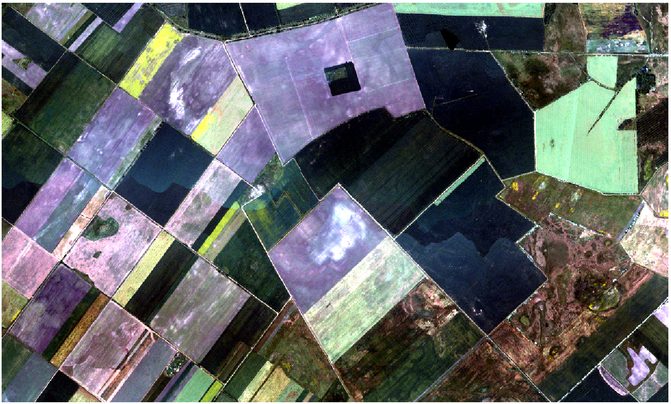
\includegraphics[width=0.7\columnwidth]{Fig/aisa.png} \\
            {\bfseries{(a)}} \\
            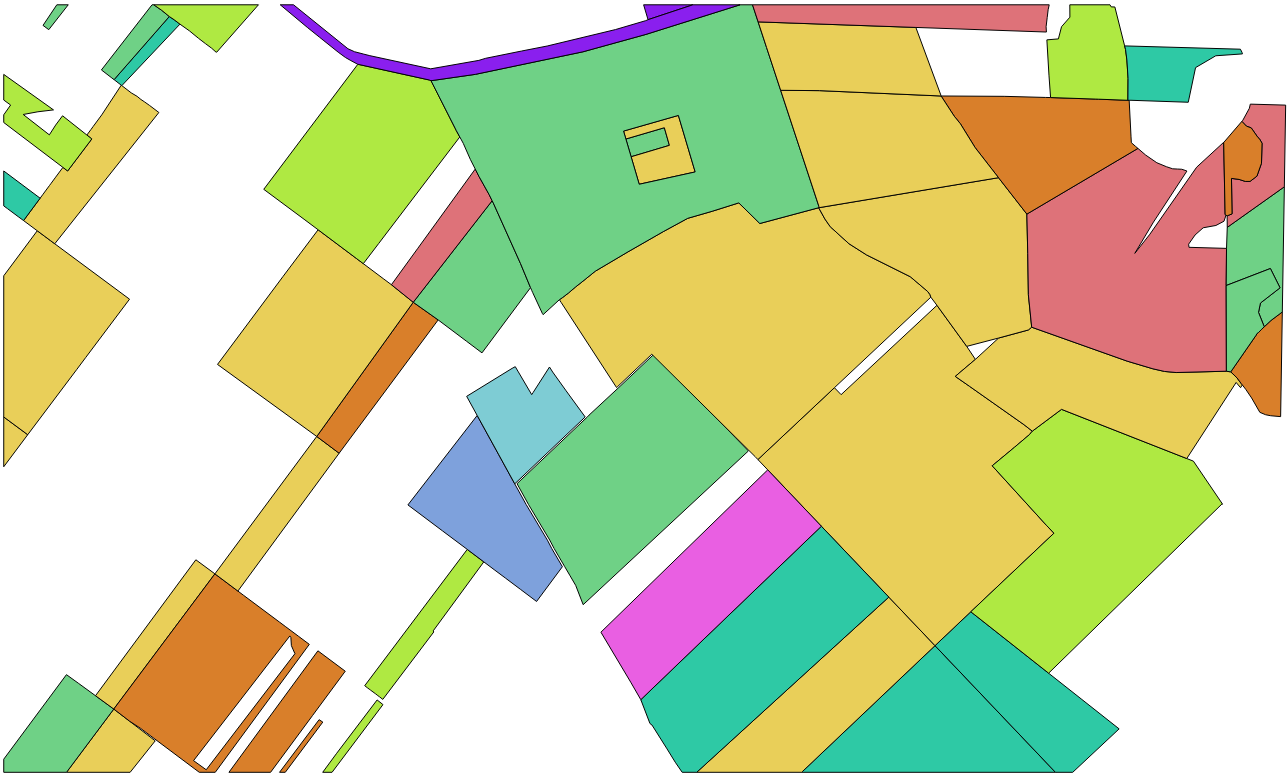
\includegraphics[width=0.7\columnwidth]{Fig/aisa_gt.png} \\
            {\bfseries{(b)}} \\
        \end{tabular}
        \caption{Aisa dataset: {\bfseries{(a)}} colored composition of the image (R: 634nm, G: 519nm, B: 477nm), {\bfseries{(b)}} groundtruth.\label{fig:aisa}}
    \end{figure}

    \begin{table}[!t]
        \centering
        \caption{Repartition of classes in Aisa dataset.\label{tab:aisa}}
        \begin{tabular}[b]{lc}\toprule
          Class & Number of samples \\ \midrule
          Winter wheat & 136,524 \\
          Sunflower & 61,517 \\
          Green fallow last year treatment & 30,197 \\
          Alfalfa & 17,626 \\
          Maize & 18,278 \\
          Millet & 7,199 \\
          Broadleaved forest & 10,746 \\
          Meadow & 23,283 \\
          Winter barley & 2,799 \\
          Reed & 4,222 \\
          Water course & 4,773 \\
          Rape & 26,566 \\
          Green fallow with shrub & 9,272 \\
          Green fallow last year treated & 3,426 \\
          Pasture & 2,107 \\
          Oat & 3,436 \\ \bottomrule
        \end{tabular}
    \end{table}

    \subsection{Potsdam dataset}
    \label{sec:pots-dataset}

    This  second dataset  is built  from a  dataset of  remote sensing
    images distributed by the International Society for Photogrammetry
    and                         Remote                         Sensing
    (ISPRS)\footnote{\url{http://www2.isprs.org/commissions/comm3/wg4/2d-sem-label-potsdam.html}}. The
    dataset is composed of aerial images of the urban area of Potsdam.
    The area is cut into 38  patches of 6000$\times$6000 pixels with a
    resolution  of 5cm  by pixel  and 4  channels are  available: Red,
    Blue, Green  and Infrared (RGBIR).   A Digital Surface  Model with
    the same  resolution is also  provided and a  so-called normalized
    DSM representing the height above  ground. The ground-truth for 24
    tiles  are   provided  with   6  classes:  Low   vegetation,  High
    vegetation, Impervious surfaces,  Buildings, Cars, Clutter.  Three
    tiles  have  been  used  in  this  work,  they  are  displayed  in
    Figure~\ref{fig:potsdam-expl}.  Table~\ref{tab:potsdam} summarizes
    the  number of  samples of  each class.

    \begin{figure}[!t]
        \centering
        \begin{tabular}{ccc}
            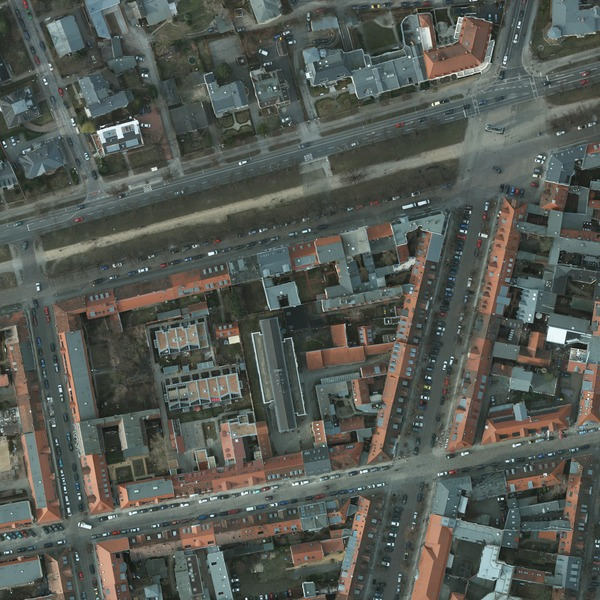
\includegraphics[width=0.3\columnwidth]{Fig/top_potsdam_5_11_RGB.jpg} &
            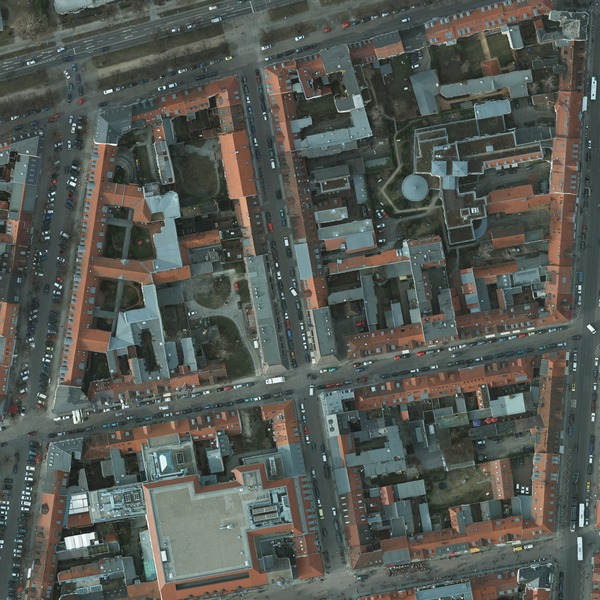
\includegraphics[width=0.3\columnwidth]{Fig/top_potsdam_5_12_RGB.jpg} &
            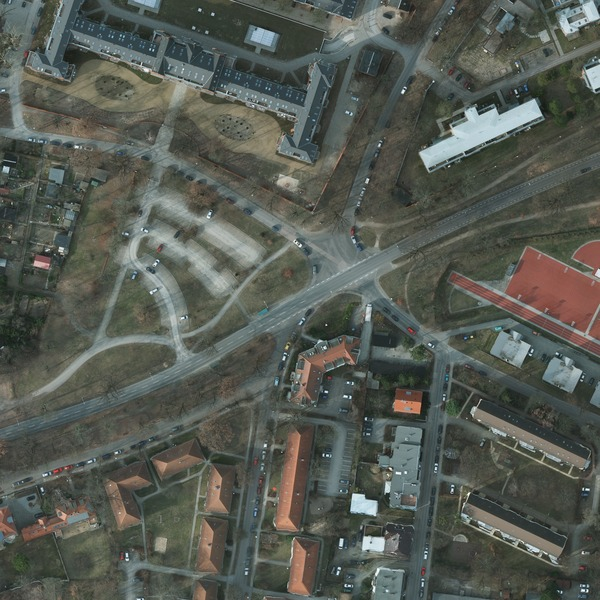
\includegraphics[width=0.3\columnwidth]{Fig/top_potsdam_3_10_RGB.jpg} \\
            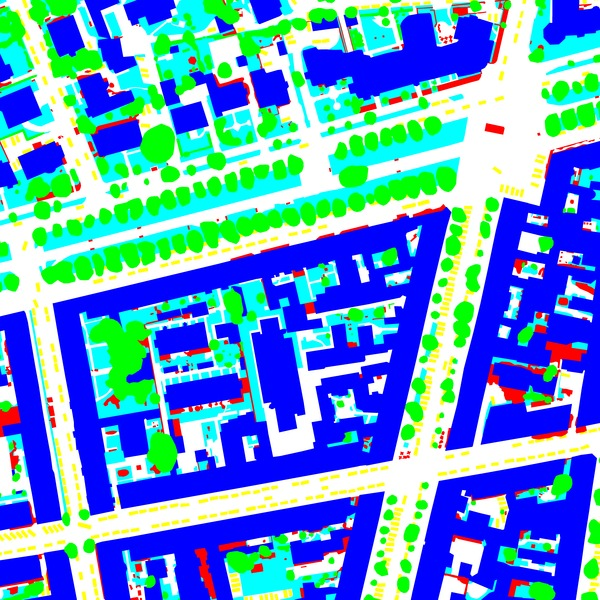
\includegraphics[width=0.3\columnwidth]{Fig/top_potsdam_5_11_label.jpg} &
            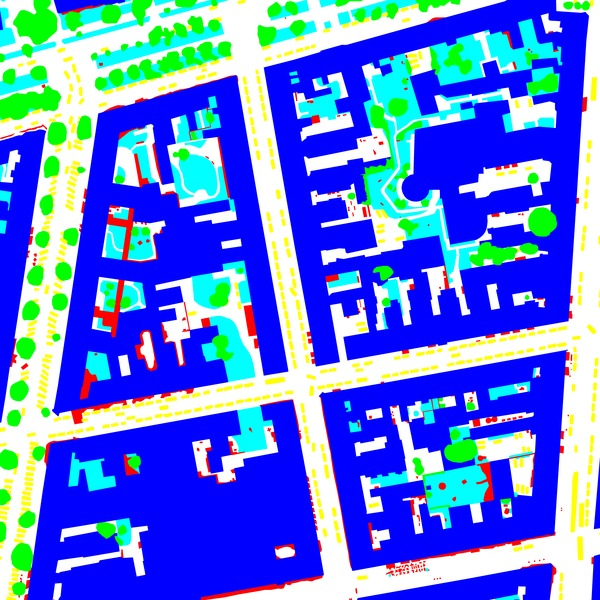
\includegraphics[width=0.3\columnwidth]{Fig/top_potsdam_5_12_label.jpg} &
            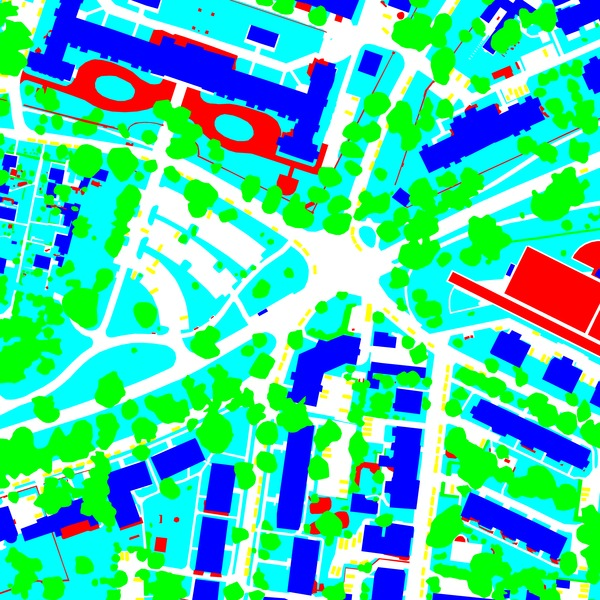
\includegraphics[width=0.3\columnwidth]{Fig/top_potsdam_3_10_label.jpg} \\
            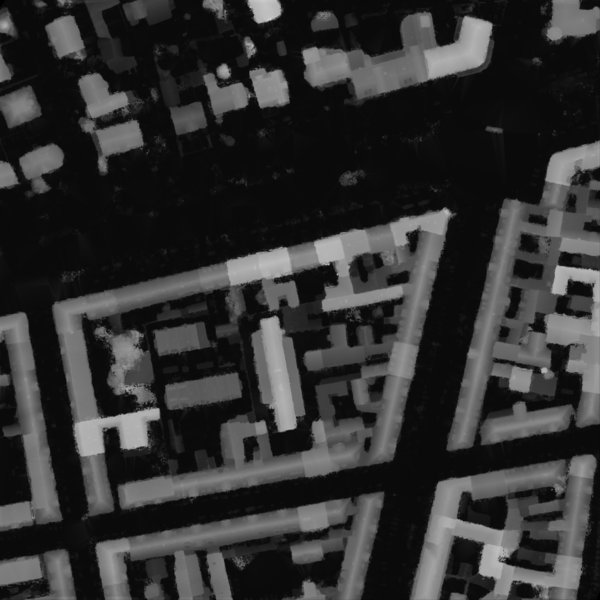
\includegraphics[width=0.3\columnwidth]{Fig/dsm_potsdam_05_11_normalized_lastools.jpg} &
            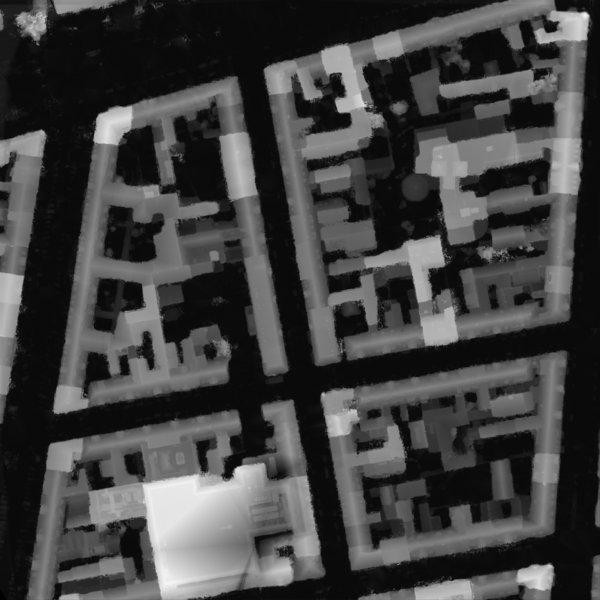
\includegraphics[width=0.3\columnwidth]{Fig/dsm_potsdam_05_12_normalized_lastools.jpg} &
            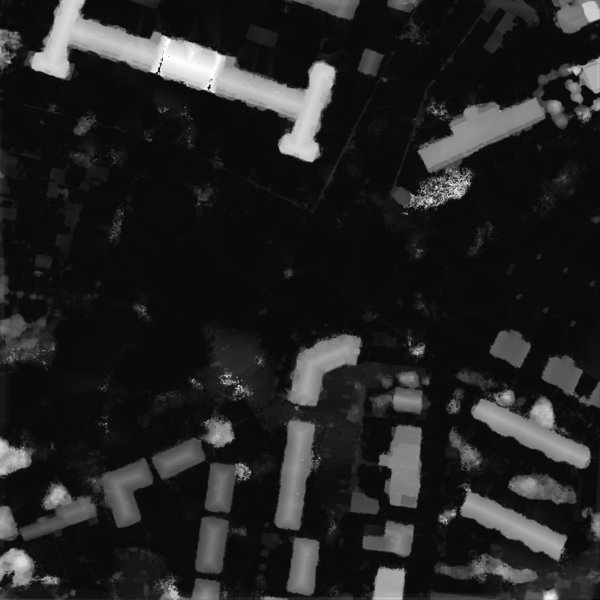
\includegraphics[width=0.3\columnwidth]{Fig/dsm_potsdam_03_10_normalized_lastools.jpg} \\
            {\bfseries{(a)}} & {\bfseries{(b)}}  & {\bfseries{(c)}}\\
        \end{tabular}
        \caption{From top to bottom, true color composition, ground-truth and normalized DSM of: {\bfseries{(a)}} tile 5\_11, {\bfseries{(b)}} tile 5\_12 and {\bfseries{(c)}} tile 3\_10.\label{fig:potsdam-expl}}
    \end{figure}

    \begin{table}[!t]
        \centering
        \caption{Repartition of classes in Aisa dataset.\label{tab:potsdam}}
        \begin{tabular}[b]{lrrr}\toprule
          Class & \# of samples in 5\_11  & \#  of samples in 5\_12  & \#  of samples in 3\_10 \\
          \midrule
          Clutter             & 1,078,611  & 812,038    & 1,890,467 \\
          Trees               & 4,493,295  & 2,132,368  & 8,780,245 \\
          Cars                & 900,076    & 1,101,541  & 434,615 \\
          Buildings           & 13,469,575 & 17,501,421 & 5,128,149 \\
          Low vegetation      & 4,718,219  & 3,210,596  & 11,428,326 \\
          Impervious surfaces & 11,340,224 & 11,242,036 & 8,338,198 \\
          \bottomrule
        \end{tabular}
    \end{table}

    In order to increase the dimensionality of the data, the following features are computed using the RGBIR images similarly to \cite{tuia2015multiclass}:
    \begin{itemize}
        \item 15 Radiometric indexes: NDVI, TNDVI, RVI, SAVI, TSAVI, MSAVI, MSAVI2, GEMI, IPVI, NDWI2, NDTI, RI, CI, BI, BI2~\cite{otb}.
        \item Morphological profile with reconstruction of each band with a disk of radius 5, 9, 13, 17, 21, 25, 29, 33, 37 and 41 (80 features)~\cite{fauvel2013advances};
        \item Attribute profile of each band with area as attribute and 1000, 2000, 5000, 10000 and 15000 as thresholds (40 features)~\cite{dalla2010morphological}.
        \item Attribute profile of each band with diagonal of bounding box as attribute and 100, 200, 500, 1000 and 20000 as thresholds (40 features)~\cite{dalla2010morphological}.
        \item Textural features with neighborhood of 19x19 pixels: mean, standard deviation, range and entropy (16 features)~\cite{otb}.
    \end{itemize}
    The normalized DSM and the raw  RGBIR image are added to these 191
    features and  then then  stacked to  create a  new image  with 196
    bands. %  The  training is  made with  tile 5\_11  and test  with two
    % tiles: 5\_12 which very similar with  tile 5\_11 and 3\_10 which a
    % further area a bit less urban and more industrial.


\section{Experimental results}
\label{sec:test}

    \subsection{Method}
    \label{sec:method}

    The aim  of the experiments is  to compare the proposed  method to
    some   standard  classifiers   used   in   operational  land   map
    production~\cite{rs70912356}. A non-optimized  previous version of
    the method has been already compared to other selection methods in
    \cite{fauvel2015fast}.  Hence,  the primary  objective is  to test
    the  operational  efficiency  and  it is  compared  to  other  OTB
    classifiers   used  operationally   through  their   command  line
    applications\footnote{\url{http://otbcb.readthedocs.io/en/latest/OTB-Applications.html}}.

    The following classifiers are tested:
    \begin{itemize}
        \item A k-nearest-neighbors classifier (KNN) with OTB default parameters (32 as number of neighbors).
        \item A Random Forest classifier with parameters optimized by gridsearch (200 trees, 40 as max depth, 50 as size of the randomly selected subset of features at each tree node)
        \item A GMM classifier with ridge regularization (GMM ridge) with regularization constant optimized by gridsearch.
    \end{itemize}
    The GMM classifier is part of the external module described in Section~\ref{sec:otb-module}.

    All these classifiers are compared with 3 configurations of the proposed GMM classifier:
    \begin{itemize}
        \item one with forward selection and JM distance as criterion (GMM SFS JM);
        \item one with forward selection and Cohen's kappa as criterion (GMM SFS kappa);
        \item one with floating forward selection and JM distance as criterion (GMM SFFS JM).
    \end{itemize}

    The training set has been created  with an equal number of samples
    for each class and additionally  a spatial stratification has been
    performed, \emph{i.e.}, each training  sample belongs to a spatial
    polygon  that  does  not  intersect  spatially  with  any  spatial
    polygons used  for the validation.   Several size of  training set
    have been tested investigated.   For the Aisa dataset, experiments
    have been conducted  using 250, 500 and 1000 samples  by class and
    for the Potsdam dataset, 1000 and 50000 samples by class.

    For SFS and  SFFS selection, the number of variables to select is set to 30 for the Aisa dataset and 60 for the Potsdam dataset. Then, a small processing is made to select the number of variables used for prediction. The evolution of the criterion function is retrieved from the model file and the discrete derivative of the criterion \emph{DJ} is computed and normalized by its maximum. The subset of variables used for classification $\Omega^{*}$ is the first subset for which this value is lower than a given threshold \emph{th}, equal  to 0.001\% in this experiment,
    \begin{equation*}
        \Omega^{*} = \Omega_{\min \{k|DJ_k<th\}}
    \end{equation*}
    with $DJ_k = \frac{J(\Omega_k) - J(\Omega_{k-1})}{\max_k (J(\Omega_k) - J(\Omega_{k-1}))}$.

    The classification  rate is presented  using Cohen's kappa  but it
    has to  be noticed the  results were  similar when looking  at the
    mean F1-score.  Processing time  has been  evaluated on  a desktop
    computer  with 4Gb  of RAM  and  Intel(R) Core(TM)  i5-3570 CPU  @
    3.40GHz $\times$ 4 processors.

    \subsection{Aisa dataset}
    \label{sec:aisa}

    When creating training and validation  sets, special care is taken
    to assure that training samples are picked out from distinct areas
    than test  samples.  The  polygons of the  reference are  split in
    smaller polygons and then 50\%  of the polygons are taken randomly
    for training and the remaining 50\% for validation.  An example of
    training      and     validation      set     is      shown     in
    Figure~\ref{fig:set-aisa}.  From the  training  polygons, a  given
    number of samples  were selected to build the  training set, while
    all  the pixels  from the  validation polygons  were used  for the
    validation.  Moreover 20  random trials were run  with a different
    training  set (different  polygons).  Table~\ref{tab:aisa-otbsimu}
    presents  the results  of the  experiment with  mean and  standard
    deviation  of  the  Kappa  coefficient  over  the  20  trials  and
    Table~\ref{tab:aisa-otbsimu-time}  the   corresponding  processing
    time.

    \begin{figure}[!t]
        \centering
        \begin{tabular}{c}
            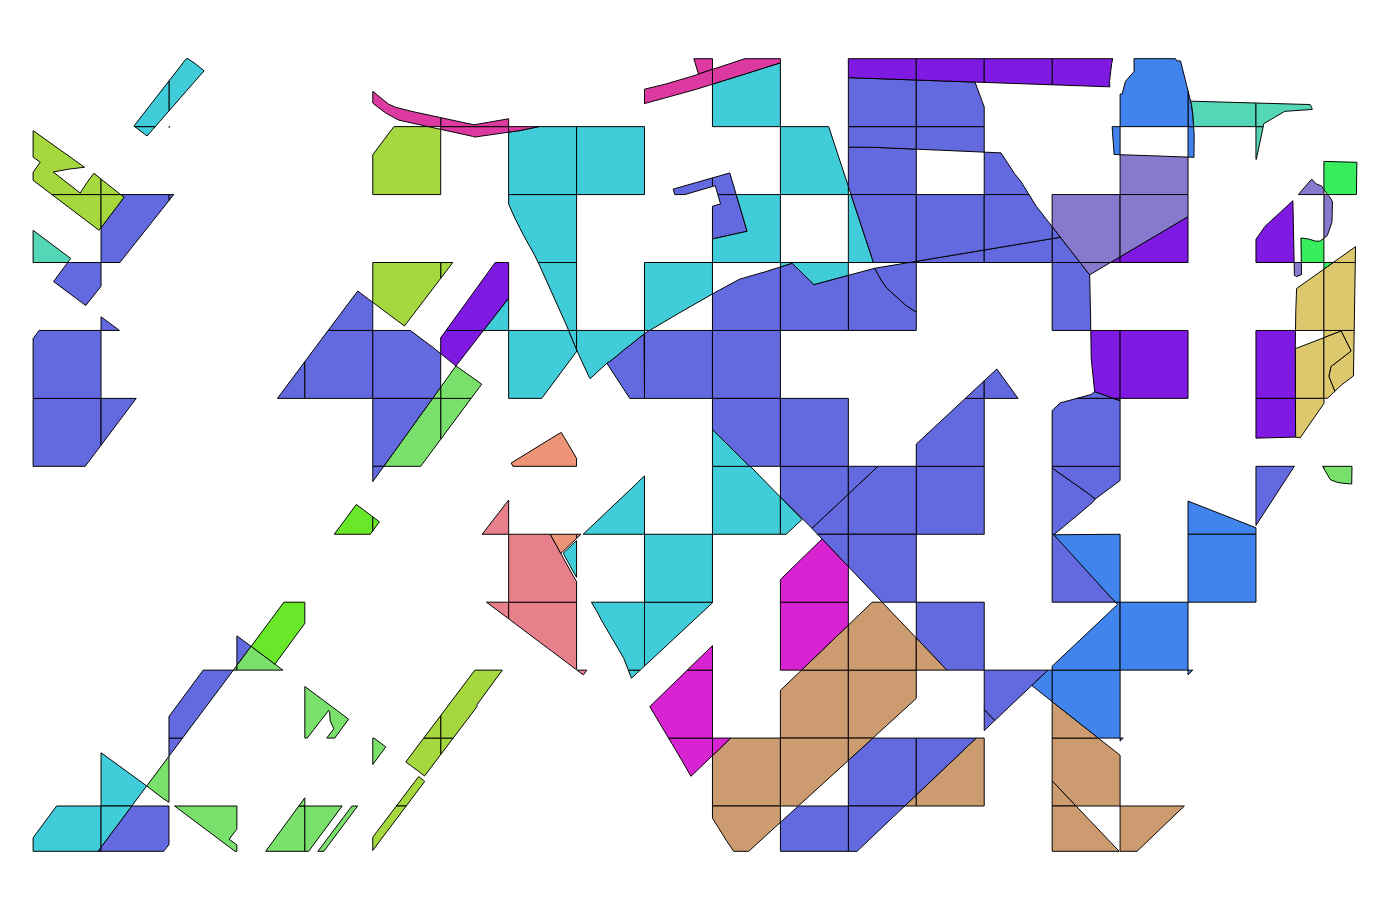
\includegraphics[width=0.7\columnwidth]{Fig/aisa_gt_train.png} \\
            {\bfseries{(a)}} \\
            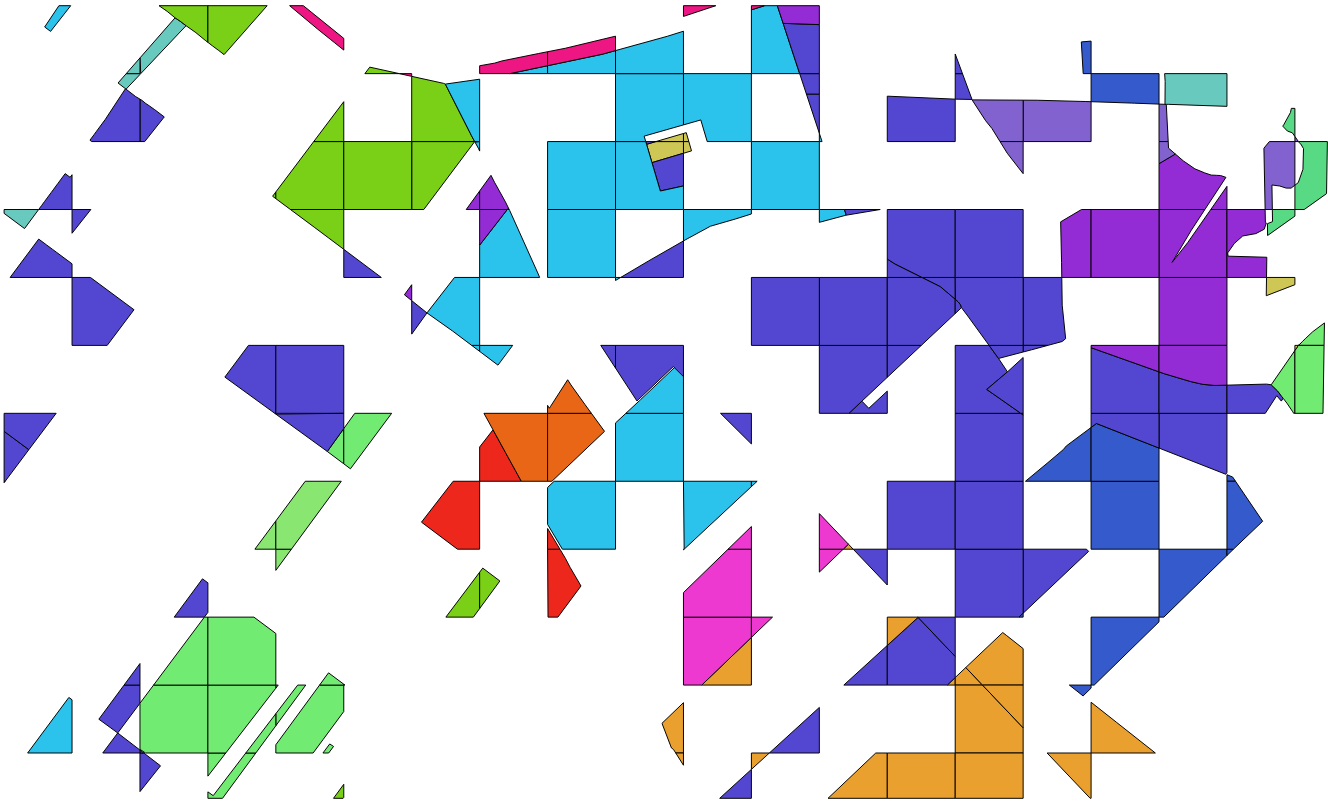
\includegraphics[width=0.7\columnwidth]{Fig/aisa_gt_test.png} \\
            {\bfseries{(b)}} \\
        \end{tabular}
        \caption{Aisa dataset: {\bfseries{(a)}} training polygons of first trial, {\bfseries{(b)}} test polygons of first trial.\label{fig:set-aisa}}
    \end{figure}

    \begin{table}[!t]
        \centering
        \caption{Average classification accuracy 20 trials (standard deviation in parenthesis).\label{tab:aisa-otbsimu}}
        \begin{tabular}{lccc}\toprule
             & \multicolumn{3}{c}{\bfseries Cohen's kappa} \\ \cline{2-4}
            \# samples by class & 250 & 500 & 1000 \\ \midrule

            GMM SFS kappa & 0.684 (0.025) & 0.698 (0.027) & 0.711 (0.028) \\
            GMM SFS JM &    0.680 (0.028) & 0.700 (0.028) & 0.710 (0.030) \\
            GMM SFFS JM &   0.680 (0.028) & 0.700 (0.028) & 0.710 (0.030) \\
            GMM ridge &     0.611 (0.040) & 0.620 (0.036) & 0.642 (0.034) \\
            KNN &           0.551 (0.035) & 0.563 (0.033) & 0.574 (0.030) \\
            Random Forest & 0.645 (0.026) & 0.673 (0.023) & 0.693 (0.023) \\
            \bottomrule
        \end{tabular}
    \end{table}

    \begin{table}[!t]
        \centering
        \caption{Mean processing time for training and classification for results in Table \ref{tab:aisa-otbsimu}.\label{tab:aisa-otbsimu-time}}
        \begin{tabularx}{\columnwidth}{l*{6}{>{\centering\arraybackslash}X}}
            \toprule
             & \multicolumn{3}{c}{\bfseries Training time (s)} & \multicolumn{3}{c}{\bfseries Classification time (s)} \\ \cline{2-7}
            \# samples by class & 250 & 500 & 1000 & 250 & 500 & 1000 \\ \midrule

            GMM SFS kappa & 257 & 496 & 955 & 7.7 & 8.6 & 8.7 \\
            GMM SFS JM &    8.6 & 8.9 & 9.1 & 9.7 & 9.8 & 9.6 \\
            GMM SFFS JM &   8.8 & 9.0 & 9.3 & 9.7 & 9.8 & 9.8 \\
            GMM ridge &     71.7 & 105 & 167 & 530 & 530 & 530 \\
            KNN &           8.9 & 19.6 & 59.7 & 387 & 639 & 887 \\
            Random Forest & 24.5 & 49.3 & 105 & 33.0 & 41.7 & 45.9 \\
            \bottomrule
        \end{tabularx}
    \end{table}

    The results show that, on this  dataset, GMM classifiers with feature selection get the best classification rate. Among the three variations of the selection algorithm, none appears to perform better than the others. Using kappa or Jeffries-Matusita distance as criterion is equal and using SFFS does not give any advantage.

    The difference with the second best classifier, Random Forest, appears to be significant when using 250 and 500 samples. Random Forest has similar performance in term of classification rate with 1000 samples. The GMM classifier with ridge regularization and the kNN classifier are both outperformed.

    In term of computational time, the GMM classifiers are as expected very fast for classification and also for training, except when the criterion function is a classification rate. In this case, using JM distance as criterion and SFS as search strategy is the best choice in term of time efficiency. The good performance in time can explain by the dimensional reduction. Actually, the decision rule corresponding to Equation~\ref{eq:decision} has a complexity in $d^3$ where $d$ is the dimension. Thus, reducing $d$ induces a reduction of the classification time.

    The processing times of the three standard classifiers suffer from the increase of training samples. For the GMM classifier with ridge, the selection of regularization parameter is more costly with more samples because the classification rate estimation needed. For the kNN classifier, the model stores all the training samples and the prediction implies to compute the distance to all the training samples which explains the increase of the processing time and additionally of the size of the model file. Finally, for the Random Forest classifier, the trees tends to be more deeper in order to capture the additional information available with more samples and that explains the increase of the processing time.
    % The computation of the kappa seems  to suffer from  a lack of  parallelization   which could be  improved. ->  plus tard dans la conclusion.

    \subsection{Potsdam dataset}

    For the Potsdam  dataset, training samples were  selected from one
    tile (5\_11)  and validation  samples were all  the pixel  of tile
    5\_12  or  3\_10.  Table~\ref{tab:potsdam-otbsimu}  presents  the
    results.

    \begin{table}[!t]
        \centering
        \caption{Kappa coefficient and processing time for 1,000 samples by class and averaged over 5 trials (standard deviation in parenthesis). Processing times are given in second.\label{tab:potsdam-otbsimu}}
        \begin{tabular}{lcccccc}\toprule
            & {\bfseries 5\_11 (train)} & {\bfseries 5\_12 (test)} & {\bfseries 3\_10 (test)} & {\bfseries Train. Time} & {\bfseries Classif. time} & {\bfseries \# of selected features} \\ \cline{2-7}
            GMM SFS kappa & 0.694 (0.002)             & {\bfseries 0.669 (0.005)} & {\bfseries 0.533 (0.008)} & 400 & 310  & 13.2 \\
            GMM SFS JM &    0.624 (0.028)             & 0.631 (0.034)             & 0.461 (0.027)             & 2   & 310  & 11 \\
            GMM SFFS JM &   0.624 (0.028)             & 0.631 (0.034)             & 0.461 (0.027)             & 2.6 & 310  & 11 \\
            GMM ridge &     0.632 (0.007)             & 0.592 (0.010)             & 0.433 (0.008)             & 10  & 2000 & all \\
            KNN &           0.637 (0.005)             & 0.607 (0.005)             & 0.478 (0.002)             &     &      & all \\
            Random Forest & {\bfseries 0.729 (0.004)} & {\bfseries 0.673 (0.005)} & {\bfseries 0.529 (0.009)} & 20  & 840  & all \\
            \bottomrule
        \end{tabular}
    \end{table}

    \begin{table}[!t]
        \centering
        \caption{Kappa coefficient and processing time for 50,000 samples by class and averaged over 5 trials (standard deviation in parenthesis). Processing times are given in second.\label{tab:potsdam-otbsimu-big}}
        \begin{tabular}{|lcccccc}\toprule
            & {\bfseries 5\_11 (train)} & {\bfseries 5\_12 (test)} & {\bfseries 3\_10 (test)} & {\bfseries Train. Time} & {\bfseries Classif. time} & {\bfseries \# of selected features} \\ \cline{2-7}
            GMM SFS kappa & 0.713 (0.001) & 0.684 (0.001) & 0.531 (0.005) & 20000 & 340 & 29 \\
            GMM SFS JM &    0.560 (0.111) & 0.576 (0.104) & 0.435 (0.085) & 6 & 330 & 10 \\
            GMM SFFS JM &   0.560 (0.111) & 0.576 (0.104) & 0.435 (0.085) & 6.6 & 340 & 10 \\
            GMM ridge &     0.641 (0.015) & 0.611 (0.026) & 0.440 (0.015) & 460 & 2000 & all \\
            Random Forest & {\bfseries 0.851 (0.001)} & {\bfseries 0.715 (0.001)} & {\bfseries 0.573 (0.002)} & 2000 & 2000 & all \\
            \bottomrule
        \end{tabular}
    \end{table}

    With this second dataset, the Random Forest classifier and the GMM classifier with kappa as selection criterion distinguished themselves by good performance. When using 1000 samples, no significant difference of classification rate has been observed on test set. But, with 50,000 samples, the Random Forest classifier better significantly better.

    It can be guessed that the fact that the Gaussian hypothesis is unlikely to be verified explains the difficulty to extract the finer information available in a larger dataset. The JM distance has stressed in Table~\ref{tab:crit} has a strong Gaussian hypothesis and the same hypotheses could also explain the drop of the classification rate of GMM classifiers with Jeffries-Matusita distance as criterion.

    The KNN classifier and the GMM classifier with ridge regularization are again outperformed even if they get more stable results than GMM classifiers with JM as criterion.

    The number of variables identified by the selection process shows that selection with JM distance as criterion identifies less relevant samples than with kappa as criterion. Moreover, the GMM classifier with kappa manages to get good performance with only 6.7\ of the variables with 1000 samples and 15\% with 50,000 samples.

    In term of processing time, results are similar than with the Aisa dataset. GMM classifiers with selection are very fast for prediction. For example, the GMM classifier with kappa as criterion is 63\% faster than the Random Forest classifier for prediction with 1000 samples and 83\% faster with 50,000 samples.

\section{Conclusion}

An algorithm for the classification of high dimension data as hyperspectral image has been presented. The classifier uses GMM model to select iteratively the most relevant features. Several variation of the algorithms has been explored. Experimentations show that allowing backward step in the selection to discard already selected features do not give significant advantages.

Additionally, from the comparison between all the measures used to rank the features, it has been shown that the Jeffries-Matusita distance can be a fast and accurate solution in some case but suffer from some limitations which remain to be determine. A possible explaination could be that this distance does not perform well when data distribution is not similar to a Gaussian distribution. More investigation is needed to confirm this hypothesis. In any case, it is possible to use directly kappa as criterion function even if it implies a loss of time.

Finally, experiments show that the developed GMM classifier performs at least as best as standard classifiers without features selection in particular Random Forest and even outperforms all of them in term of classification time. The next step would be to compare to other feature selection methods.

The second achievement of this work is the development of an efficient implementation using GMM properties to derive fast update rules of the model. The resulting code is available as a remote module of the Orfeo toolbox on Github and make it possible to process huge quantity of high dimension data.

Finally, an improvement could be made to increase the stability of the selected features. For example, with hyperspectral data, a selection of continuous intervals and not band is a possible solution which has already been explored in \cite{serpico2007extraction}.

The python and C++ code are available freely for download: \url{https://github.com/Laadr/FFFS}, \url{https://github.com/Laadr/otbExternalFastFeaturesSelection}.

\appendices
\section{}
\label{app:proof-update}
\subsection{Proof of update rules}
    \subsubsection{Proposition~\ref{eq:update-inv-back}}
        \begin{proof}
            \begin{align*}
                \mathbf{A} - \alpha \mathbf{v} \mathbf{v}^t
                &= (\boldsymbol{\Sigma}^{(k-1)})^{-1} + \frac{1}{\alpha} (\boldsymbol{\Sigma}^{(k-1)})^{-1} \mathbf{u} \mathbf{u}^t (\boldsymbol{\Sigma}^{(k-1)})^{-1} \\
                &~~~- \alpha (- \frac{1}{\alpha} (\boldsymbol{\Sigma}^{(k-1)})^{-1} \mathbf{u}) (- \frac{1}{\alpha} \mathbf{u}^t (\boldsymbol{\Sigma}^{(k-1)})^{-1})) \\
                &= (\boldsymbol{\Sigma}^{(k-1)})^{-1}
            \end{align*}
        \end{proof}

    \subsubsection{Proposition~\ref{eq:update-quad}}
        \begin{proof}
            \begin{align*}
                (&\mathbf{x}^{(k)})^t (\boldsymbol{\Sigma}^{(k)})^{-1} \mathbf{x}^{(k)}
                = \left[\begin{array}{cc} (\mathbf{x}^{(k-1)})^t   & x_k \end{array}\right]
                \left[\begin{array}{cc}
                \mathbf{A}   & \mathbf{v} \\
                \mathbf{v}^t & \frac{1}{\alpha}
                \end{array}\right]
                \left[\begin{array}{c} \mathbf{v} \\ x_k \end{array}\right] \\
                &= \left[\begin{array}{cc} (\mathbf{x}^{(k-1)})^t \mathbf{A} + x_k \mathbf{v}^t & (\mathbf{x}^{(k-1)})^t \mathbf{v} + \frac{x_k}{\alpha} \end{array}\right]
                \left[\begin{array}{c} \mathbf{v} \\ x_k \end{array}\right] \\
                &= (\mathbf{x}^{(k-1)})^t \mathbf{A} \mathbf{x}^{(k-1)} + x_k \mathbf{v}^t \mathbf{x}^{(k-1)} + (\mathbf{x}^{(k-1)})^t \mathbf{v} x_k + \frac{(x_k)^2}{\alpha} \\
                &= (\mathbf{x}^{(k-1)})^t ((\boldsymbol{\Sigma}^{(k-1)})^{-1} + \frac{1}{\alpha} (\boldsymbol{\Sigma}^{(k-1)})^{-1} \mathbf{u} \mathbf{u}^t (\boldsymbol{\Sigma}^{(k-1)})^{-1}) \mathbf{x}^{(k-1)}\\
                &~~~+ 2 x_k \mathbf{v}^t \mathbf{x}^{(k-1)} + \frac{(x_k)^2}{\alpha} \\
                &= (\mathbf{x}^{(k-1)})^t ((\boldsymbol{\Sigma}^{(k-1)})^{-1} + \alpha \mathbf{v} \mathbf{v}^t) \mathbf{x}^{(k-1)}\\
                &~~~+ 2 x_k \mathbf{v}^t \mathbf{x}^{(k-1)} + \frac{(x_k)^2}{\alpha} \\
                &= (\mathbf{x}^{(k-1)})^t (\boldsymbol{\Sigma}^{(k-1)})^{-1} \mathbf{x}^{(k-1)} + \alpha ( (\mathbf{x}^{(k-1)})^t \mathbf{v} \mathbf{v}^t \mathbf{x}^{(k-1)} \\
                &~~~+ 2 \frac{x_k}{\alpha} \mathbf{v}^t \mathbf{x}^{(k-1)} + \frac{(x_k)^2}{\alpha^2}) \\
                &= (\mathbf{x}^{(k-1)})^t (\boldsymbol{\Sigma}^{(k-1)})^{-1} \mathbf{x}^{(k-1)} + \alpha ( (\mathbf{x}^{(k-1)})^t \mathbf{v} + \frac{x_k}{\alpha} )^2 \\
                &= (\mathbf{x}^{(k-1)})^t (\boldsymbol{\Sigma}^{(k-1)})^{-1} \mathbf{x}^{(k-1)} + \alpha ( \left[\begin{array}{cc} \mathbf{v}^t & \frac{1}{\alpha} \end{array}\right] \mathbf{x}^{(k)} )^2
            \end{align*}
        \end{proof}

% \section*{Acknowledgment}

% The authors would like to thank...

\bibliographystyle{IEEEtran}
\bibliography{biblio}

% biography section
%
% If you have an EPS/PDF photo (graphicx package needed) extra braces are
% needed around the contents of the optional argument to biography to prevent
% the LaTeX parser from getting confused when it sees the complicated
% \includegraphics command within an optional argument. (You could create
% your own custom macro containing the \includegraphics command to make things
% simpler here.)
%\begin{IEEEbiography}[{\includegraphics[width=1in,height=1.25in,clip,keepaspectratio]{mshell}}]{Michael Shell}
% or if you just want to reserve a space for a photo:

\begin{IEEEbiography}{Michael Shell}
Biography text here.
\end{IEEEbiography}

% if you will not have a photo at all:
\begin{IEEEbiographynophoto}{John Doe}
Biography text here.
\end{IEEEbiographynophoto}

% insert where needed to balance the two columns on the last page with
% biographies
%\newpage

\end{document}



%\begin{figure}[!t]

% An example of a double column floating figure using two subfigures.
% (The subfig.sty package must be loaded for this to work.)
% The subfigure \label commands are set within each subfloat command,
% and the \label for the overall figure must come after \caption.
% \hfil is used as a separator to get equal spacing.
% Watch out that the combined width of all the subfigures on a
% line do not exceed the text width or a line break will occur.
%
%\begin{figure*}[!t]
%\centering
%\subfloat[Case I]{\includegraphics[width=2.5in]{box}%
%\label{fig_first_case}}
%\hfil
%\subfloat[Case II]{\includegraphics[width=2.5in]{box}%
%\label{fig_second_case}}
%\caption{Simulation results for the network.}
%\label{fig_sim}
%\end{figure*}
%
% Note that often IEEE papers with subfigures do not employ subfigure
% captions (using the optional argument to \subfloat[]), but instead will
% reference/describe all of them (a), (b), etc., within the main caption.
% Be aware that for subfig.sty to generate the (a), (b), etc., subfigure
% labels, the optional argument to \subfloat must be present. If a
% subcaption is not desired, just leave its contents blank,
% e.g., \subfloat[].


% An example of a floating table. Note that, for IEEE style tables, the
% \caption command should come BEFORE the table and, given that table
% captions serve much like titles, are usually capitalized except for words
% such as a, an, and, as, at, but, by, for, in, nor, of, on, or, the, to
% and up, which are usually not capitalized unless they are the first or
% last word of the caption. Table text will default to \footnotesize as
% the IEEE normally uses this smaller font for tables.
% The \label must come after \caption as always.
%
%\begin{table}[!t]
%% increase table row spacing, adjust to taste
%\renewcommand{\arraystretch}{1.3}
% if using array.sty, it might be a good idea to tweak the value of
% \extrarowheight as needed to properly center the text within the cells
%\caption{An Example of a Table}
%\label{table_example}
%\centering
%% Some packages, such as MDW tools, offer better commands for making tables
%% than the plain LaTeX2e tabular which is used here.
%\begin{tabular}{|c||c|}
%\hline
%One & Two\\
%\hline
%Three & Four\\
%\hline
%\end{tabular}
%\end{table}


% Note that the IEEE does not put floats in the very first column
% - or typically anywhere on the first page for that matter. Also,
% in-text middle ("here") positioning is typically not used, but it
% is allowed and encouraged for Computer Society conferences (but
% not Computer Society journals). Most IEEE journals/conferences use
% top floats exclusively.
% Note that, LaTeX2e, unlike IEEE journals/conferences, places
% footnotes above bottom floats. This can be corrected via the
% \fnbelowfloat command of the stfloats package.
%%% Local Variables:
%%% mode: latex
%%% TeX-master: t
%%% End:
